\cleardoublepage
%https://www3.ntu.edu.sg/home/ehchua/programming/java/datarepresentation.html
\chapter{Software Model}
The RX algorithm has been chosen for this work because it is the benchmark for this kind of algorithms \cite{borghys_hyperspectral_2012}, \cite{rosario_semiparametric_2012}, \cite{matteoli_tutorial_2010} and many existing algorithms basing on RX in some manner.
\\
In order to become familiar with the algorithm and create a platform where tests can be easily performed, a software implementation has been made as a first step.
\\
The first step is to divide the algorithm into simpler operations:
\begin{itemize}
\item Calculate the mean, deviation and K covariance matrix of the image
\item Calculate $K^{-1}$ that is, the inverse of the covariance matrix
\item Calculate $\delta ^{RX}$ for each pixel in the image
\item Sort the results
\end{itemize}
\pagebreak
\subsection{Mean, deviation and covariancce matrix}
One of the bottlenecks in this type of FPGA-based systems is the input and output of data \cite{tang_multi-fpga_2014}. Since the calculations of mean, variance and covariance matrix need the original matrix -a cube- for this, it has been decided to calculate these in a CPU and transmit the results to the FPGA. In addition, the operations are relatively simple for a CPU. Next, the pseudocode of the three is presented.
\\
\algnewcommand{\LineComment}[1]{\State \(\triangleright\) #1}
\begin{algorithm}
  \caption{Pseudocode for the mean, deviation and covariance matrix}
  \begin{algorithmic}[1]
    \LineComment{$bands$ : number of bands in the image}
    \LineComment{$pixels$ : number of pixels in the image}
    \LineComment{$A$ : the image in the form of a 2D matrix with $pixels \times bands$}
    \LineComment{$^T$ is used to denote the transpose of a matrix}
    \Statex
    \Function{mean}{$A$}
      %\State{$mean[bands]$}
      \For{$i \gets 0 \textrm{ to } bands-1$}
      	\State{$sum \gets 0$}
      	\For{$j \gets 0 \textrm{ to } pixels-1$}
       		\State{$sum \gets sum + A[i][j]$}
      	\EndFor
      	\State{$mean[i] \gets sum/pixels$}
      \EndFor
      \Return{$mean$}
    \EndFunction
    
    \Statex
    
    \Function{deviation}{$A, mean$}
    
      \Return{$A^T - mean$} \Comment{This operation is a matrix subtraction}
    \EndFunction
    
    \Statex
    
    \Function{covariance}{$deviation$}
    
      \Return{$deviation^T * deviation / (pixels-1)$}
    \EndFunction
  \end{algorithmic}
\end{algorithm}

The covariance, a $band^2$ matrix is then transmitted to the FPGA to calculate its inverse.
\clearpage

\subsection{Inverse}
\subsubsection{Choosing the algorithm}
Before starting the implementation, several algorithms to perform the inverse have been studied.
\paragraph{QR Factorization\citep{alberto_oliveira_de_souza_junior_exploration_2020}:}
QR factorization breaks down the $A$ matrix into the product of two matrices $A = QR$, with $Q$ being an orthogonal matrix and $R$ a superior triangular matrix. With this triangular matrix it becomes easy to calculate the inverse. However, although QR factorization can be efficiently performed on a powerful matrix multiplication module or several modules that can be executed simultaneously, such as in a GPU, it does not take advantage of the capabilities provided by our system such as arbitrary width arithmetic units.
\paragraph{Gauss Jordan elimination method\cite{gonzalez_fpga_2016}:}
The Gauss Jordan method dictates that if we have a $A$ matrix that can be transformed into the identity matrix through elementary operations, these same operations transform the identity matrix into $A^{-1}$. Since it is possible to execute these elementary operations in an entire row at once and the operations between rows are independent, this method is easily parallelizable.
Therefore, this was the chosen method.
\\
\\
Generally speaking, the execution of the algorithm takes place in such a way that:
\begin{enumerate}
\item An identity matrix is generated
\item The same operations are performed on both matrices until the $A$ matrix is transformed into the identity matrix
\item The result is in the matrix generated in the first step
\end{enumerate}
\noindent As seen in the following pseudocode, these elementary operations are performed in 3 steps:
\\
\\
\begin{algorithm}
  \caption{Pseudocode of the Gauss Jordan method}
  \begin{algorithmic}[1]
    %\Require{$A$ is a square matrix with the size $n*n$}
    \State{$A$ : a square matrix with the size $n*n$}
    \State{$A^{-1}$ : an identity matrix with the size $n*n$}
    \Statex
    \Function{inverse}{$A$}
      \For{$i \gets 0 \textrm{ to } n-1$} \Comment{Forward elimination to build the upper trangular matrix}
      \LineComment{row $i$ acts as the pivot}
      \If{$A[i][i] = 0$}   \Comment{If the later divisor is 0}
      	\For{$j \gets i+1 \textrm{ to } n-1$}
      		\If{$A[i][j] \neq 0$}
       			\State{$A[i] \gets A[j],\ A[j] \gets A[i]$}
      		\EndIf
      	\EndFor
      \EndIf
      \For{$j \gets 0 \textrm{ to } n-1$}
        \State{$A^{-1}[j] \gets A^{-1}[j]-A^{-1}[i]*(A[j][i]/A[i][i])$}
        \State{$A[j] \gets A[j]-A[i]*(A[j][i]/A[i][i])$}
        \Comment{These two operations may run in parallel}
      \EndFor
      \LineComment{After a complete iteration of the outer loop, the pivot contains the desired form}
      \EndFor
      \\
      \\
      \For{$i \gets n-1 \textrm{ to } 0$} \Comment{Backward elimination to build a diagonal matrix}
      \For{$j \gets i-1 \textrm{ to } 0$}
        \State{$A^{-1}[j] \gets A^{-1}[j]-A^{-1}[i]*(A[j][i]/A[i][i])$}
        \State{$A[j] \gets A[j]-A[i]*(A[j][i]/A[i][i])$}
        \Comment{These two operations may run in parallel}
      \EndFor
      \EndFor
      \\
      \\
      \For{$i \gets 0 \textrm{ to } n-1$} \Comment{Last division to build identity matrix}
        \State{$A^{-1}[i] \gets A^{-1}[i]*(1/A[i][i])$}
        \State{$A[i] \gets A[i]*(1/A[i][i])$}
        \LineComment{There is no need to update the values in the starting matrix}
      \EndFor
      \Return{$A^{-1}$}
    \EndFunction
  \end{algorithmic}
\end{algorithm}

It is also possible to calculate the inverse directly for each row, performing the three steps consecutievly in a row, but this way limits the parallelization between different rows.

\clearpage

\subsection{Matrix multiplication}
With the inverse of the convariance matrix calculated in the FPGA, the real RX algorithm can continue to be performed, where a hyperspectral pixel is multiplied with this inverse. This calculation will require the CPU to transmit the original image, the original image next to the average, or the deviation already calculated to the FPGA.
\\
\noindent The RX algorithm dictates that:
\[ rx(x) = (x-\mu)^{T} K^{-1}_{N \times N} (x-\mu) \]


\indent \(K^{-1}_{N \times N}\) \ \ \ being the inverse matrix with a dimension of \(N \times N\),\\
\indent \((x-\mu)\) \ \	being the deviation of a pixel a dimension of \(N \times 1\) and \\			
\indent \((x-\mu)^{T}\) \ it's transpose, with a dimension of \(1 \times N\).\\

\noindent In this step, the inverse matrix gets effectively multiplied by a unique pixel across all bands. Through row reduction, a single value for this pixel is recovered which can then be mapped to a 2d image.\\

Since the operands are heterogeneous, use can be made of the associative law on matrix products that dictates that:
	\[A * (B * C) = (A * B) * C\]
	to optimize the operation.\\


\paragraph{}
\phantomsection
\label{alternativa}
In the implementation sectiona study on what alternative to use will be carried out, as this depends heavily on the hardware architecture.

\section{Adapting the arithmetic}
As shown before in \autoref{fig:fp}, floating point arithmetic operations are very inefficient compared to fixed point operations. In the next chapter a transformation strategy will be defined and the steps followed to make this transition will be shown.
\\
\\
Taking advantage that the RX algorithm only needs relative and not exact values, ie, the highest value found in the results will be the most anomalous -see \ref{mayor}- regardless of whether it exceeds a certain threshold or not, the fixed-point representation may be simplified by ignoring the fractional part and keeping only the integer.

\subsection{DSP Blocks}
The DSP blocks are prefabricated circuits found next to the FPGA logic and implement arithmetic operations. These blocks allow to perform operations more efficiently and operate at higher frequencies than equivalent logic in the fabric, besides not occupying space in it. However, as they are prefabricated blocks, they do not offer the same flexibility as the rest of the FPGA logic. This implies that the size of the operands and the cost of operation resources will not always be proportionally related. Therefore, different widths have been tested and their resource usage has been noted. The results of these tests for multiplication are in the following table:

\begin{center}
 \begin{tabular}{|c c |c|} 
 \hline
 Width operand A & Width operand B & DSP48 Slices used \\ [0.5ex] 
 \hline\hline
 25 & 18 & 1 \\ 
 \hline
 35 & 25 & 2 \\
 \hline
 52 & 24 & 3 \\
 \hline
 42 & 35 & 4 \\
 \hline
 64 & 25 & 4 \\
 \hline
 52 & 42 & 6 \\
 \hline
\end{tabular}
\end{center}
Depending on the width of the operands, the operation will use a different amount of resources (data obtained for signed multiplication in Vivado 2019.2 on Xilinx Series 7 plates)
\\
\\
For subtraction operations up to 48bits, only one DSP is used, so they are not expected to require more than one block.
\\
The divisions cannot be implemented by this type of blocks, so they will use standard logic and can be used with an arbitrary width.
\\
\\
With this data for all the operations that are going to be carried out in the FPGA is recorded.
\\
\\
A hardware model implemented in software was used to determine the width of the multiplications. This model truncates both the input and output operands of each operation. The final results correspond then to the ratio of anomalies that are between the first x, up to 30.
\begin{figure}[h!]
\centering
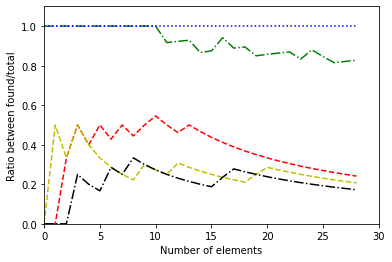
\includegraphics[height=2.5in]{figures/width.png}
\caption{Ratio of anomalies found in the first x using different bit widths for the multiplication. Dataset: Hydice}
  \label{fig:width}
\end{figure}

Como se puede observar en \autoref{fig:width}, ESTO TENGO QUE REPETIRLO.
\\

\subsection{Improving accuracy}
It is also necessary to create rules to shift the results to maintain the highest possible accuracy without producing overflow.
\\
For example, the divisions made in the inverse calculation produce very small numbers where the fractional part is relevant to the final result. Since this part is lost in integer arithmetic, it is necessary to multiply the operands to produce results where the point is shifted to the left. These multiplications will always be done in powers of 2, negative if required to decrease the bit width, as they are trivial to implement in an FPGA and do not require resources.
\\
\\
The results indicated that the greatest loss of accuracy occurred in the inverse calculation. Therefore, the model was revised and shifts were included in the initial matrix capture, in the initialization in the case of $A^{-1}$ and in the transfer to the FPGA in the case of $A$. Different shifts were also included for each phase of the inverse.


